% =============================================================================
% FSE 2027 Industry Papers -- revision of Middleware '26 Industrial Track #71.
% Long paper limit: 10 pages of text and figures + 2 pages of references.
% Every new result is a \tbd cell or a \TODOdata{} slot; each one names the
% data/*.csv file that fills it (protocol: experiment-protocol.md).
% \TODOcheck{} marks statements about the internal prototype that the team must
% confirm against SaaG-P before submission.
% =============================================================================
\documentclass[sigconf,screen]{acmart}

\usepackage{booktabs}
\usepackage{amsmath}
\usepackage{microtype}
\usepackage{array}
\usepackage{tabularx}
\usepackage{url}
\usepackage{tikz}
\usetikzlibrary{arrows.meta, positioning, fit, backgrounds, shapes.geometric}

\settopmatter{printacmref=false}
\setcopyright{none}
\renewcommand\footnotetextcopyrightpermission[1]{}
\pagestyle{plain}

\acmConference[FSE Companion '27]{35th ACM Symposium on the Foundations of Software Engineering}{July 12--16, 2027}{Shenzhen, China}
\acmBooktitle{Companion Proceedings of the 35th ACM Symposium on the Foundations of Software Engineering (FSE '27), July 12--16, 2027, Shenzhen, China}
\acmYear{2027}
\acmDOI{}
\acmISBN{}

\setlength{\tabcolsep}{3pt}
\newcolumntype{Y}{>{\raggedright\arraybackslash}X}

% ---- draft markers (remove before submission) -------------------------------
\newcommand{\TODOdata}[1]{\textcolor{red}{\textbf{[TODO(data): #1]}}}
\newcommand{\TODOcheck}[1]{\textcolor{orange}{\textbf{[TODO(check): #1]}}}
\newcommand{\tbd}{\textcolor{red}{\textbf{?}}}
% -----------------------------------------------------------------------------

\begin{document}

\title[Gating Pub/Sub Misconfigurations in CI/CD]{Gating Publish/Subscribe Misconfigurations in CI/CD with an Architectural Graph Model: Experience from a Naval Combat Management System}

\author{Ibrahim Onuralp Yigit}
\affiliation{%
  \institution{Command Control and Defense Technologies, HAVELSAN}
  \city{Istanbul}
  \country{Turkiye}
}
\email{iyigit@havelsan.com.tr}

\author{Onurcan Ersen}
\affiliation{%
  \institution{Command Control and Defense Technologies, HAVELSAN}
  \city{Istanbul}
  \country{Turkiye}
}
\email{oersen@havelsan.com.tr}

\author{Mustafa Can Caliskan}
\affiliation{%
  \institution{Command Control and Defense Technologies, HAVELSAN}
  \city{Istanbul}
  \country{Turkiye}
}
\email{mccaliskan@havelsan.com.tr}

\author{Emre Karagoz}
\affiliation{%
  \institution{Software Development Center, TNRCC}
  \city{Istanbul}
  \country{Turkiye}
}
\email{karagoz.e5926@dzkk.tsk.tr}

\author{Omer Kursat Ucarer}
\affiliation{%
  \institution{Software Development Center, TNRCC}
  \city{Istanbul}
  \country{Turkiye}
}
\email{ucarer.o1595@dzkk.tsk.tr}

\begin{abstract}
A naval combat management system (CMS) is hundreds of applications exchanging data over DDS-style publish/subscribe middleware. Its costliest integration defects are architectural misconfigurations that no unit test sees: a data writer that offers weaker Quality-of-Service (QoS) than its reader requests and is therefore never matched, a topic left without subscribers after a refactor, a dependency cycle that deadlocks start-up, a host whose cores are over-committed. Today these surface at shipyard integration or sea trials.

We report on SaaG, a CI/CD gate built at HAVELSAN that rebuilds each candidate release as a typed dependency graph from its configuration descriptors, checks it against middleware rules, and blocks builds that introduce new severe violations. We evaluate it four ways: injecting 12 classes of faulty and 7 classes of benign mutations into five generated platform profiles, with QoS verdicts cross-checked against the middleware's own endpoint matching; running it on a fielded baseline whose findings two architects triaged; replaying \tbd{} historical integration defects; and timing it. The gate detects \tbd{} of the injected faults within its implemented rules at a false-positive rate of \tbd{}, flags \tbd{} of \tbd{} historical defects, and adds 16--100\,s to a build. The binding constraint was not analysis but data: one baseline drew on \tbd{} configuration sources in \tbd{} formats and took \tbd{} person-weeks to curate. We report what that means for organizations adopting such gates.
\end{abstract}

\begin{CCSXML}
<ccs2012>
<concept><concept_id>10011007.10011074.10011099</concept_id><concept_desc>Software and its engineering~Software verification and validation</concept_desc><concept_significance>500</concept_significance></concept>
<concept><concept_id>10011007.10010940.10010971.10011120</concept_id><concept_desc>Software and its engineering~Distributed systems organizing principles</concept_desc><concept_significance>300</concept_significance></concept>
</ccs2012>
\end{CCSXML}
\ccsdesc[500]{Software and its engineering~Software verification and validation}
\ccsdesc[300]{Software and its engineering~Distributed systems organizing principles}
\TODOcheck{verify CCS concept ids at dl.acm.org/ccs}

\keywords{publish/subscribe middleware, DDS QoS, architecture conformance, configuration errors, CI/CD gating, fault injection, defense systems}

\maketitle

% =============================================================================
\section{Introduction}
% =============================================================================

Naval combat management systems (CMS) used to be monolithic mainframe software. Today they are open, distributed architectures: radar trackers, track fusion, threat evaluation, weapon assignment, fire control and operator consoles run as separate applications on mission computers and consoles, and exchange data over publish/subscribe middleware that follows the OMG Data Distribution Service (DDS) model~\cite{omg2015dds}. The CMS we work on, developed by HAVELSAN with the Turkish Naval Forces Research Center Command, serves surface combatants, amphibious ships, unmanned vehicles and maritime patrol aircraft, with hundreds of applications per platform.

Continuous integration~\cite{humble2010} checks each of these applications well and their composition poorly. Unit and component tests run one application at a time, so a class of defects passes every test and only appears when the whole system is assembled:
\begin{itemize}
\item \emph{QoS mismatch.} In DDS, a reader states the QoS it \emph{requests} and a writer the QoS it \emph{offers}; if the offer is weaker (e.g., the weapon assignment writer offers \texttt{VOLATILE} durability while fire control requests \texttt{TRANSIENT\_LOCAL}), the middleware never connects them. No exception is raised; data simply never arrives.
\item \emph{Orphaned topic.} A refactor removes the last subscriber of a topic that another subsystem still publishes, or vice versa.
\item \emph{Dependency cycle.} Two subsystems each wait for the other's data at start-up and deadlock the console.
\item \emph{Core over-commitment.} Real-time applications pinned to a host request more cores than the host has.
\end{itemize}
Finding these needs the assembled target: consoles, mission computers, sensor and weapon simulators. That hardware cannot sit in a CI pipeline, so the defects are found at shipyard integration, harbor acceptance tests (HAT) or sea acceptance tests (SAT), where each costs days of a scarce test window.

\emph{SaaG} (System as a Graph) moves these checks into the pipeline. On each merge request it rebuilds the candidate release as a typed graph from configuration descriptors---which application runs where, publishes and subscribes to what, with which QoS---derives who depends on whom, checks rules over that graph, and fails the build when the candidate adds a severe violation. It reuses the graph model of Yigit and Buzluca~\cite{yigit2025graph}; what is new here is the gate built on it and the evidence about it.

Showing that such a gate is cheap does not show that it is useful. This paper therefore asks:
\begin{description}
\item[RQ1] Does the gate detect injected misconfigurations, and does it accept valid changes?
\item[RQ2] What does it report on a real fielded baseline, and are those findings real?
\item[RQ3] Would it have caught defects that historically escaped to integration and sea trials?
\item[RQ4] What does it cost in the pipeline?
\end{description}

\noindent\textbf{Contributions.}
\begin{enumerate}
\item A CI/CD gate for DDS-style pub/sub systems (\S3): a rule catalog over request/offered QoS, partitions, topic continuity, dependency cycles and core capacity; a severity rubric adapted from MIL-STD-882E~\cite{milstd882e}; and gate semantics for a legacy codebase (fail-closed policy, delta-aware gating, waiver register). Table~\ref{tab:delta} separates this from what~\cite{yigit2025graph} provides.
\item An effectiveness evaluation (\S4--\S5): fault injection with an independent middleware oracle, a triaged fielded baseline, historical defect replay, cost, and a sensitivity analysis of the severity rubric.
\item Evidence on the real adoption barrier (\S6): configuration data is spread across organizational and security silos, and acquiring it---not analyzing it---dominated the effort. We quantify that effort and give recommendations.
\end{enumerate}

\noindent\textbf{Deployment status.} SaaG runs as a CLI gate on a GitLab CI runner over hand-curated JSON descriptors exported from application repositories. It is not yet fed from an authoritative configuration source; \S6 explains why. We distinguish throughout between rules the prototype implements and capabilities that are specified but not built.

% =============================================================================
\section{Background and Running Example}
% =============================================================================

\subsection{DDS QoS matching in one paragraph}
DDS applications exchange typed samples on named \emph{topics}. Each data writer and data reader carries QoS policies. For a subset of policies, the specification defines a \emph{request/offered} (RxO) rule: a writer and a reader are matched only if what the writer offers is at least what the reader requests~\cite{omg2015dds}. For \texttt{DURABILITY} the order is \texttt{VOLATILE} $<$ \texttt{TRANSIENT\_LOCAL} $<$ \texttt{TRANSIENT} $<$ \texttt{PERSISTENT}; for \texttt{RELIABILITY}, \texttt{BEST\_EFFORT} $<$ \texttt{RELIABLE}; \texttt{DEADLINE}, \texttt{LATENCY\_BUDGET}, \texttt{LIVELINESS}, \texttt{OWNERSHIP} and \texttt{DESTINATION\_ORDER} are RxO as well. \texttt{PARTITION} is not ordered: writer and reader must share a partition name. An unmatched pair is reported only through an incompatible-QoS status that applications must poll or listen for---in practice, rarely---so the failure is silent. Middleware tools show these statuses at run time, which for a CMS means on a testbed or on the ship.

\subsection{The industrial setting}
The CMS middleware is proprietary but follows the DDS data-centric model and RxO semantics, so we use DDS terms throughout. A platform baseline is the set of application versions, their hosts and their middleware configuration for one ship class. Configuration lives in many places: application repositories, middleware QoS profiles, start-up scripts, interface control documents (ICDs) for sensors and weapons, and shipyard commissioning archives (\S6). Five platform classes, from a single-node maritime patrol aircraft to a corvette with distributed consoles, define our evaluation subjects (\S4.1).

\subsection{Running example}
Figure~\ref{fig:example} follows one change through the gate. Three applications run on two hosts: \emph{Track Fusion} (TF) publishes \texttt{track}; \emph{Weapon Assignment} (WA) subscribes to \texttt{track} and publishes \texttt{engagement\_order}; \emph{Fire Control} (FC) subscribes to \texttt{engagement\_order} and requests \texttt{TRANSIENT\_LOCAL} durability so that it receives the current order even if it restarts. A merge request changes WA's writer to \texttt{VOLATILE}. Every unit test of WA still passes.

SaaG reads the candidate's descriptors (a), builds the structural graph (b), and projects dependency edges in the direction failures propagate---FC depends on WA because FC starves if WA stops, not the reverse (c). The RxO rule compares FC's request with WA's offer on \texttt{engagement\_order}, finds the offer weaker, and, because the channel is tagged safety-critical, rates the violation S1. The violation is absent from the baseline, so the gate exits 1 and the merge request is blocked with the message in (d).

\begin{figure*}[t]
\centering
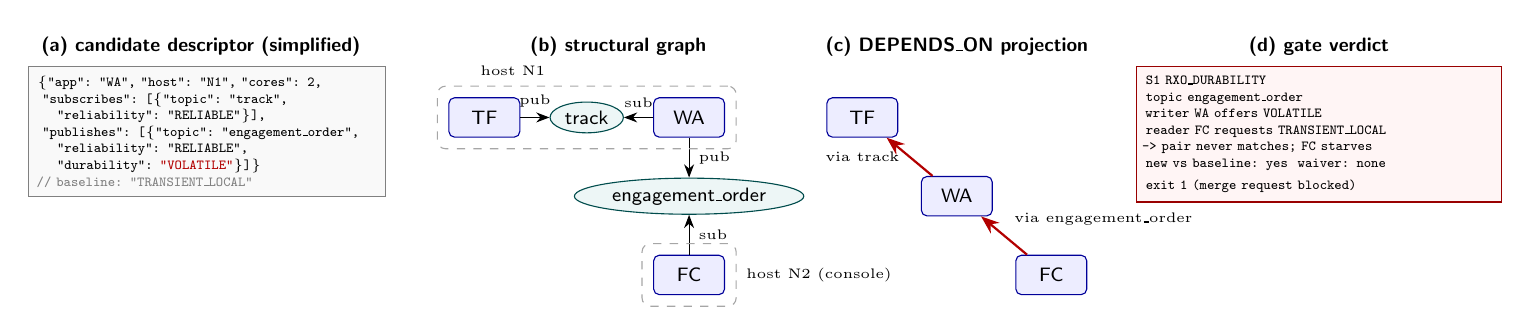
\begin{tikzpicture}[font=\sffamily\scriptsize, >=Stealth,
  app/.style={draw=blue!60!black, fill=blue!7, rounded corners=2pt, minimum width=0.9cm, minimum height=0.5cm},
  top/.style={draw=teal!60!black, fill=teal!7, ellipse, inner sep=1.5pt},
  host/.style={draw=gray!70, dashed, rounded corners=3pt, inner sep=4pt},
  dep/.style={->, thick, red!70!black},
  lab/.style={font=\sffamily\bfseries\scriptsize}]

% (a) descriptor
\node[lab] (la) at (0,2.1) {(a) candidate descriptor (simplified)};
\node[draw=gray, fill=gray!5, align=left, font=\ttfamily\tiny, anchor=north west, text width=4.3cm] at (-2.2,1.85) {%
\{"app": "WA", "host": "N1", "cores": 2,\\
\ "subscribes": [\{"topic": "track",\\
\ \ \ \ "reliability": "RELIABLE"\}],\\
\ "publishes": [\{"topic": "engagement\_order",\\
\ \ \ \ "reliability": "RELIABLE",\\
\ \ \ \ "durability": \textcolor{red!70!black}{"VOLATILE"}\}]\}\\
\textcolor{gray}{// baseline: "TRANSIENT\_LOCAL"}};

% (b) structural graph
\node[lab] at (5.3,2.1) {(b) structural graph};
\node[app] (tf) at (3.6,1.2) {TF};
\node[top] (t1) at (4.9,1.2) {track};
\node[app] (wa) at (6.2,1.2) {WA};
\node[top] (t2) at (6.2,0.2) {engagement\_order};
\node[app] (fc) at (6.2,-0.8) {FC};
\draw[->] (tf) -- node[above, font=\tiny]{pub} (t1);
\draw[->] (wa) -- node[above, font=\tiny]{sub} (t1);
\draw[->] (wa) -- node[right, font=\tiny]{pub} (t2);
\draw[->] (fc) -- node[right, font=\tiny]{sub} (t2);
\node[host, fit=(tf)(wa), label={[font=\tiny]above left:host N1}] {};
\node[host, fit=(fc), label={[font=\tiny]right:host N2 (console)}] {};

% (c) dependency projection
\node[lab] at (9.6,2.1) {(c) DEPENDS\_ON projection};
\node[app] (tf2) at (8.4,1.2) {TF};
\node[app] (wa2) at (9.6,0.2) {WA};
\node[app] (fc2) at (10.8,-0.8) {FC};
\draw[dep] (wa2) -- node[left, font=\tiny, text=black]{via track} (tf2);
\draw[dep] (fc2) -- node[above right, font=\tiny, text=black, align=left]{via engagement\_order} (wa2);

% (d) verdict
\node[lab] at (14.2,2.1) {(d) gate verdict};
\node[draw=red!60!black, fill=red!4, align=left, font=\ttfamily\tiny, anchor=north, text width=4.4cm] at (14.2,1.85) {%
S1 RXO\_DURABILITY\\
topic engagement\_order\\
writer WA offers VOLATILE\\
reader FC requests TRANSIENT\_LOCAL\\
-> pair never matches; FC starves\\
new vs baseline: yes \ waiver: none\\[2pt]
\textbf{exit 1 (merge request blocked)}};
\end{tikzpicture}
\caption{Running example. A one-field change in a writer's QoS (a) passes unit tests. SaaG builds the structural graph (b), projects failure dependencies opposite to data flow (c), finds the request/offered durability violation on a safety-critical channel, and blocks the merge request (d).}
\label{fig:example}
\end{figure*}

% =============================================================================
\section{SaaG: Model, Rules and Gate}
% =============================================================================

\subsection{Graph model (from~\cite{yigit2025graph})}
SaaG represents a platform baseline as a typed directed multigraph $G=(V,E,\tau_V,\tau_E)$. Vertices are \emph{applications}, \emph{brokers} (middleware routing services), \emph{topics}, \emph{hosts} (mission computers, consoles, server chassis) and shared \emph{libraries}. Structural edges are read directly from descriptors: \texttt{PUBLISHES\_TO}, \texttt{SUBSCRIBES\_TO}, \texttt{ROUTES}, \texttt{RUNS\_ON}, \texttt{CONNECTS\_TO} and \texttt{USES}.

Message flow runs from publisher to subscriber, but failure dependency runs the other way: if a publisher stops, its subscribers starve; if a subscriber stops, the publisher is unaffected. Six projection rules (Table~\ref{tab:dep_rules}) derive \texttt{DEPENDS\_ON} edges from the structural edges. The cycle rule (\S3.2) runs on these projected edges, and diagnostic mode (\S3.5) uses them to report what a change can affect.

Each vertex also carries a criticality weight $w(v)\in[0,1]$, computed in~\cite{yigit2025graph} from the QoS of the topics it touches, message size and fan-out. In the gate the weights do one thing: they order findings \emph{within} a severity level for triage. They do not decide pass or fail; \S5.6 tests how sensitive triage order and severities are to them. \TODOcheck{confirm against protocol decision D2 that weights only order triage; if they feed severity, rewrite this paragraph}

\begin{table}[t]
\centering
\caption{\texttt{DEPENDS\_ON} projection rules (from~\cite{yigit2025graph}). $X \to Y$ means $X$ depends on $Y$.}
\label{tab:dep_rules}
\small
\begin{tabularx}{\columnwidth}{c l Y}
\toprule
\# & Type & Derived when \\
\midrule
1 & app $\to$ app & $B$ subscribes to a topic that $A$ publishes ($B \to A$) \\
2 & app $\to$ broker & $A$ publishes or subscribes to a topic that broker $R$ routes \\
3 & host $\to$ host & Rule 1 lifted to the hosts of $B$ and $A$ \\
4 & host $\to$ broker & Rule 2 lifted to the host of $A$ \\
5 & app $\to$ library & $A$ links library $\ell$ (\texttt{USES}) \\
6 & broker $\to$ broker & Two brokers share a host \\
\bottomrule
\end{tabularx}
\end{table}

\begin{table}[t]
\centering
\caption{What this paper adds to the graph model of~\cite{yigit2025graph}.}
\label{tab:delta}
\small
\begin{tabularx}{\columnwidth}{Y c c}
\toprule
Element & \cite{yigit2025graph} & This paper \\
\midrule
Entity/edge types, \texttt{DEPENDS\_ON} projection & $\bullet$ & reused \\
QoS-derived criticality weights & $\bullet$ & reused for triage order \\
Candidate isolation $G_{u'}$ per merge request & & $\bullet$ \\
Middleware rule catalog (Table~\ref{tab:rules}) & & $\bullet$ \\
Severity rubric adapted from MIL-STD-882E & & $\bullet$ \\
Gate semantics: exit codes, fail-closed, delta-aware, waivers & & $\bullet$ \\
Effectiveness evaluation (RQ1--RQ3) & & $\bullet$ \\
Data-acquisition study & & $\bullet$ \\
\bottomrule
\end{tabularx}
\end{table}
\TODOcheck{confirm the split in Table 2 with the RASSE'25 paper; adjust if any rule was introduced there}

\subsection{Rules, as implemented}
Table~\ref{tab:rules} lists the rules the prototype runs, stated at the granularity at which they are actually implemented. The narrowings matter, and RQ1 measures their cost: the RxO rule compares QoS per \emph{topic}, not per writer--reader pair \TODOcheck{state exactly how a topic's offer and request are aggregated}; the schema rule matches topic names, not message fields; the core rule checks that requested cores fit host capacity, not that core masks do not overlap.

\begin{table}[t]
\centering
\caption{Rules implemented in the prototype (SaaG-P).}
\label{tab:rules}
\small
\begin{tabularx}{\columnwidth}{l Y l}
\toprule
Rule & Check, as implemented & Typical sev. \\
\midrule
RxO & Per topic: offered $\ge$ requested for \texttt{DURABILITY}, \texttt{RELIABILITY}; shared \texttt{PARTITION} \TODOcheck{D1: + DEADLINE, LIVELINESS, \ldots?} & S1--S2 \\
Continuity & Topic with no publisher or no subscriber & S2--S3 \\
Schema & Publisher and subscriber agree on the topic name & S2 \\
Cycle & Strongly connected component (Tarjan) in \texttt{DEPENDS\_ON} among applications & S2 \\
Capacity & $\sum$ requested cores of units on a host $\le$ host cores & S1--S3 \\
\bottomrule
\end{tabularx}
\end{table}

\subsection{Severity}
MIL-STD-882E~\cite{milstd882e} grades the severity of mishaps, not of configuration defects, so we adapt its four levels: a violation is rated by the worst credible mishap it could contribute to, given which channels and hosts it touches. Channels and hosts carry a safety-criticality tag maintained by the system safety team. \TODOcheck{D2: state the exact mapping}
\begin{itemize}
\item \textbf{S1} --- loss of a safety-critical function (e.g., unmatched pair on a weapon engagement channel; over-committed fire control host).
\item \textbf{S2} --- loss of a mission-essential function with redundancy or mitigation (e.g., orphaned data-link forwarding topic; cycle among engagement planning units).
\item \textbf{S3} --- non-critical anomaly (e.g., orphaned auxiliary sensor stream).
\item \textbf{S4} --- maintenance warning (e.g., deprecated library version).
\end{itemize}
Severity is deliberately independent of the middleware's transport priority: a low-priority channel can still feed a safety-critical function.

\subsection{Gate semantics}
For each merge request, SaaG substitutes the candidate version $u'$ of the changed unit into the baseline inventory, giving an isolated candidate graph $G_{u'}$; the baseline is never modified. The gate exits 0 (pass; S3/S4 logged), 1 (an S1 or S2 violation; pipeline aborted) or 2 (the descriptors could not be parsed or analyzed). On safety-critical branches the gate is \emph{fail-closed}: exit 2 also aborts, so an unanalyzable candidate never passes unverified.

A legacy baseline already carries violations, and an absolute gate would block every build. SaaG therefore gates on the \emph{delta}: a candidate is blocked only if $\mathrm{Viol}(G_{u'})\setminus\mathrm{Viol}(G_{\mathrm{base}})$ contains an S1/S2 violation. Known baseline violations live in a waiver register; each waiver is approved by the chief architect, signed, and expires.

\subsection{Diagnostic mode}
The same graph serves architects outside the pipeline: SCCs show cycles to break; orphaned topics and unreferenced libraries show configuration debt; high-weight brokers and topics show where a change has wide reach; and a proposed change can be applied to a copy of the baseline graph to see what it affects. \S5.3 reports what this surfaced on a fielded baseline and what the team did with it.

% =============================================================================
\section{Study Design}
% =============================================================================

\subsection{Subjects}
\noindent\textbf{Generated profiles.} Operational configuration data of fielded combat systems is not releasable, and \S6 explains why it was also hard to obtain internally. We therefore generate five platform profiles whose scale parameters---application, topic, host and library counts, and the distributions of QoS settings and fan-out---were elicited from the architects of the corresponding platforms: Maritime Surveillance Aircraft (1 host), Coastal Surveillance (25), Unmanned Surface Vehicle (1), Amphibious Ship (65) and Corvette (20). They span 180--320 applications, 1{,}200--2{,}800 topics and 1{,}500--3{,}300 vertices. Each profile is generated with 5 seeds, giving 25 baselines. Generated baselines are violation-free by construction; we confirm this with the gate (\S5.2).

\noindent\textbf{Platform R.} One fielded platform baseline, anonymized as \emph{Platform R} under the clearance recorded in our data package: \TODOdata{clearance.md -- anonymization sentence}. Its descriptors were curated by hand from the sources described in \S6.

\noindent\textbf{Historical defects.} \tbd{} architectural defects drawn from the program's defect tracker by a selection rule fixed before running the gate: \TODOdata{rq3\_replay.csv -- selection\_rule}.

\subsection{RQ1: fault injection}
Each mutant applies one mutation to one clean baseline (Table~\ref{tab:mutants}). Faulty operators M1--M12 cover the fault classes the rules target, plus three that target the known narrowings of Table~\ref{tab:rules} (M10--M12), so the cost of each narrowing is measured rather than asserted. Benign operators B1--B7 make changes a correct gate must accept. Mutation sites are drawn uniformly, stratified so that at least a third lie on safety-critical channels. We generate 40 mutants per operator per profile (200 per operator).

A finding counts as a detection only if it is \emph{at} the mutated element; findings elsewhere count as false positives. We report per-operator recall and false-positive rate with Wilson 95\% intervals, gate-decision accuracy (exit 1 exactly when the expected severity is S1/S2), and severity agreement.

\noindent\textbf{Oracle.} For the QoS operators, our expected outcome is our own reading of the specification. To check that reading independently, we instantiate 50 sampled writer--reader pairs per operator in \TODOdata{rq1\_oracle.csv -- middleware} and record whether the middleware reports incompatible QoS and whether the pair matches.

\begin{table}[t]
\centering
\caption{Mutation operators. Exp.: expected outcome on SaaG-P ($+$ detect; $\times$ known miss; $\checkmark$ accept).}
\label{tab:mutants}
\small
\begin{tabularx}{\columnwidth}{l Y c}
\toprule
Op & Mutation & Exp. \\
\midrule
M1 & Writer durability below a reader's request & $+$ \\
M2 & \texttt{BEST\_EFFORT} writer, \texttt{RELIABLE} reader & $+$ \\
M3 & Redundant publisher moved to another \texttt{PARTITION} & $+$ \\
M4 & Offered \texttt{DEADLINE} period longer than requested & \TODOcheck{D1} \\
M5 & Offered \texttt{LIVELINESS} weaker than requested & \TODOcheck{D1} \\
M6 / M7 & Last subscriber / last publisher of a topic removed & $+$ \\
M8 & Dependency edge closing a cycle (length 2, 3, $\ge$5) & $+$ \\
M9 & Requested cores on a host exceed capacity & $+$ \\
M10 & Overlapping core masks within capacity & $\times$ \\
M11 & Same topic name, different message fields & $\times$ \\
M12 & One of several writers on a topic weakened & $+$/? \\
\midrule
B1 / B2 & Writer QoS raised / reader QoS lowered & $\checkmark$ \\
B3 & Compatible subscriber added & $\checkmark$ \\
B4 / B5 & Consistent rename / reordering of descriptors & $\checkmark$ \\
B6 & Unit moved to a host with spare cores & $\checkmark$ \\
B7 & Edge added that closes no cycle & $\checkmark$ \\
\bottomrule
\end{tabularx}
\end{table}

\subsection{RQ2: fielded baseline}
We run the gate on Platform R without baseline subtraction. Two architects triage each finding independently (on a sample of at least 30 findings) as \emph{TP-fix} (real; fixed or scheduled), \emph{TP-debt} (real; accepted into the waiver register), \emph{FP-model} (the rule is wrong for this case) or \emph{FP-data} (a descriptor was wrong or stale); we report Cohen's $\kappa$ and resolve disagreements jointly. We then replay the last \tbd{} merged change sets with absolute and with delta-aware gating and count blocks under each.

\subsection{RQ3: historical replay}
For each selected defect, we reconstruct the pre-fix descriptors, run the gate, and record whether it flags the defect, with which rule and severity, and---if not---why: capability not implemented, information absent from descriptors, or outside the gate's scope.

\subsection{RQ4 and sensitivity}
Latency is the mean of 500 evaluations per profile across the 5 seeds after 20 warm-up runs, on Ubuntu 22.04 (AMD EPYC 7763, 32\,GB), Python 3.11, NetworkX 3.2, in memory. For sensitivity, we perturb each weight parameter and QoS factor value by $\pm$10\% and $\pm$20\% one at a time, plus 200 random joint perturbations within $\pm$20\%, and measure on the RQ1 mutants and on Platform R how many severities change, how many gate decisions flip, and Kendall's $\tau$ between triage orders.

% =============================================================================
\section{Results}
% =============================================================================

\subsection{Overview}
\TODOdata{two-sentence summary of RQ1--RQ4 once all files are filled}

\subsection{RQ1: detection and acceptance}
\TODOdata{rq1\_mutants.csv -- clean baselines: number of findings on the 25 unmutated baselines and their cause}

Table~\ref{tab:rq1} gives the results per operator. \TODOdata{rq1\_mutants.csv -- recall of implemented rules (M1--M3, M6--M9), pooled with CI; FP rate on B1--B7}

\TODOdata{rq1\_mutants.csv -- M10--M12: measured miss rates; for M12, how often the flagged writer was the mutated one}

\TODOdata{rq1\_oracle.csv -- agreement with the middleware; list and explain every disagreement}

\begin{table}[t]
\centering
\caption{RQ1 results, pooled over 5 profiles $\times$ 5 seeds ($n=200$ per operator). Recall and FP rate with Wilson 95\% CI. \TODOdata{rq1\_mutants.csv}}
\label{tab:rq1}
\small
\begin{tabularx}{\columnwidth}{l Y c c c}
\toprule
Op & Rule & Recall & Gate acc. & Sev. agr. \\
\midrule
M1 & RxO & \tbd & \tbd & \tbd \\
M2 & RxO & \tbd & \tbd & \tbd \\
M3 & RxO (partition) & \tbd & \tbd & \tbd \\
M4 / M5 & RxO (extended) & \tbd & \tbd & \tbd \\
M6 / M7 & Continuity & \tbd & \tbd & \tbd \\
M8 & Cycle & \tbd & \tbd & \tbd \\
M9 & Capacity & \tbd & \tbd & \tbd \\
M10 & (non-overlap, not impl.) & \tbd & \tbd & \tbd \\
M11 & (field schema, not impl.) & \tbd & \tbd & \tbd \\
M12 & RxO, per topic & \tbd & \tbd & \tbd \\
\midrule
 & & FP rate & Gate acc. & \\
\midrule
B1--B7 & all & \tbd & \tbd & \\
clean & all & \tbd & \tbd & \\
\bottomrule
\end{tabularx}
\end{table}

\subsection{RQ2: findings on Platform R}
\begin{table}[t]
\centering
\caption{RQ2: absolute audit of Platform R, with architect triage. \TODOdata{rq2\_baseline\_findings.csv}}
\label{tab:rq2}
\small
\begin{tabularx}{\columnwidth}{Y c c c c c}
\toprule
Rule & Findings & TP-fix & TP-debt & FP-model & FP-data \\
\midrule
RxO & \tbd & \tbd & \tbd & \tbd & \tbd \\
Continuity & \tbd & \tbd & \tbd & \tbd & \tbd \\
Schema & \tbd & \tbd & \tbd & \tbd & \tbd \\
Cycle & \tbd & \tbd & \tbd & \tbd & \tbd \\
Capacity & \tbd & \tbd & \tbd & \tbd & \tbd \\
\midrule
Total & \tbd & \tbd & \tbd & \tbd & \tbd \\
\bottomrule
\end{tabularx}
\end{table}
\TODOdata{rq2\_baseline\_findings.csv -- precision on Platform R; Cohen's $\kappa$; median triage minutes; what the FP-model findings have in common}

\TODOdata{rq2\_delta\_gating.csv -- of \tbd{} change sets, blocked under absolute vs. delta-aware gating; how many delta blocks were justified; waiver entries created}

\noindent\textbf{Diagnostic mode.} \TODOdata{rq2\_diagnostic\_outcomes.csv -- SCCs, orphaned topics, unreferenced libraries found, and what was actually refactored or ticketed. Report only outcomes that happened.}

\subsection{RQ3: historical defects}
\begin{table}[t]
\centering
\caption{RQ3: replay of historical defects. Found: phase in which the defect was found. \TODOdata{rq3\_replay.csv}}
\label{tab:rq3}
\small
\begin{tabularx}{\columnwidth}{l Y l c Y}
\toprule
ID & Fault class & Found & Flagged & Rule / reason missed \\
\midrule
D1 & \tbd & \tbd & \tbd & \tbd \\
D2 & \tbd & \tbd & \tbd & \tbd \\
\ldots & & & & \\
\bottomrule
\end{tabularx}
\end{table}
\TODOdata{rq3\_replay.csv -- flagged k of n; for the misses, which were implementation gaps (Table~\ref{tab:gap}) vs. missing data vs. out of scope; cost bucket of flagged defects}

\subsection{RQ4: cost}
Table~\ref{tab:latency} gives gate latency. On the generated profiles the gate takes 15.5\,s (single-host aircraft profile) to 100.2\,s (corvette), P95 $\le$ 102.3\,s. Graph construction is 52--72\% of it; rule evaluation and dependency projection the rest. Latency grows with vertex and edge count; the 65-host amphibious profile is slower than its size alone suggests because rules 3--4 lift dependencies across many hosts. Against the program's release pipeline, which takes about 30 minutes (\TODOdata{rq4\_latency.csv -- full\_pipeline: n and window}), the gate adds at most 5.6\%. \TODOdata{rq4\_latency.csv -- Platform R latency}

\begin{table}[t]
\centering
\caption{RQ4: gate latency (s). Generated rows: mean of 500 runs over 5 seeds; counts approximate.}
\label{tab:latency}
\small
\setlength{\tabcolsep}{2.2pt}
\begin{tabularx}{\columnwidth}{Y r r r r r r}
\toprule
Profile & Hosts & $|V|$ & $|E|$ & Constr. & Total & P95 \\
\midrule
Maritime Surv. Aircraft & 1 & 1500 & 4800 & 11.11 & 15.53 & 17.27 \\
Coastal Surveillance & 25 & 2200 & 7100 & 24.49 & 38.57 & 38.94 \\
Unmanned Surface Veh. & 1 & 2200 & 7000 & 23.53 & 45.42 & 47.63 \\
Amphibious Ship & 65 & 2800 & 9600 & 44.52 & 85.87 & 87.68 \\
Corvette & 20 & 3300 & 11500 & 52.34 & 100.16 & 102.31 \\
\midrule
Platform R & \tbd & \tbd & \tbd & \tbd & \tbd & \tbd \\
\bottomrule
\end{tabularx}
\end{table}

\subsection{Sensitivity of severity and triage}
\TODOdata{sens\_weights.csv -- fraction of severities changed and gate decisions flipped under $\pm$10/20\% and joint perturbation; Kendall $\tau$ of triage order. If severity does not depend on weights (D2), state that gate decisions are invariant by construction and report only $\tau$.}

% =============================================================================
\section{Industrial Experience: Data, Not Analysis, Is the Bottleneck}
% =============================================================================

RQ4 shows the analysis is cheap. Building the input was not. This section reports what it took to curate Platform R's descriptors and why the prototype is still not fed automatically.

\subsection{Where configuration lives}
The information one baseline needs is split across three kinds of silo. \emph{Engineering silos}: application code and some QoS settings live in Git, but QoS is also set in middleware XML profiles, in code, and in start-up scripts, with no single authoritative form. \emph{Security and contractual silos}: sensor and weapon ICDs and the hardware core bindings are held in shipyard commissioning archives under separate release control, some owned by subcontractors. \emph{Inventory silos}: the enterprise asset database is built for manual audit and has no machine-readable export, so a CI runner cannot ask it what a target host looks like.

Table~\ref{tab:effort} quantifies the cost for Platform R. \TODOdata{lessons\_effort.csv -- number of sources and formats; fields reconciled by hand and conflicts found; person-weeks; access lead times; approvals refused}

\begin{table}[t]
\centering
\caption{Data acquisition for Platform R. \TODOdata{lessons\_effort.csv}}
\label{tab:effort}
\small
\begin{tabularx}{\columnwidth}{Y c c c}
\toprule
Source & Format & Lead time (d) & Conflicts \\
\midrule
Application repositories & \tbd & \tbd & \tbd \\
Middleware QoS profiles & \tbd & \tbd & \tbd \\
Start-up scripts / core bindings & \tbd & \tbd & \tbd \\
Sensor/weapon ICDs & \tbd & \tbd & \tbd \\
Asset database & \tbd & \tbd & \tbd \\
\midrule
Total curation effort & \multicolumn{3}{c}{\tbd{} person-weeks} \\
\bottomrule
\end{tabularx}
\end{table}

\noindent\textbf{Curation itself found defects.} \TODOdata{lessons\_effort.csv -- descriptor\_errors\_found: inconsistencies between sources discovered while building the model, and whether any were real configuration errors}

\noindent\textbf{Organizational obstacles.} \TODOdata{lessons\_effort.csv -- notes: which approvals were needed, who owned which source, which requests were refused or delayed, and how that shaped what the prototype could check}

\subsection{What the silos cost in capability}
Table~\ref{tab:gap} lists the capabilities our architects specified, what the prototype realizes, what blocks the rest, and---new in this version---what that gap costs as measured in \S5. Six of seven gaps are blocked by data, not by algorithms: each missing capability is a check we know how to write but cannot feed.

\begin{table*}[t]
\centering
\caption{Specified vs. realized capabilities, their blockers, and the measured consequence.}
\label{tab:gap}
\footnotesize
\begin{tabularx}{\textwidth}{l l Y Y}
\toprule
Specified capability & Realized in SaaG-P & Blocker & Measured consequence \\
\midrule
1. Endpoint-level RxO matching & Per-topic & \textbf{Data:} endpoint QoS held in vendor tool chains & M12 (\S5.2): \tbd \\
2. Field-level schema alignment & Topic-name match & \textbf{Data:} sensor/weapon ICD parsers not on the CI runner & M11: \tbd \\
3. Core mask non-overlap & Host capacity & \textbf{Data:} core bindings in scripts outside application repos & M10: \tbd; RQ3: \tbd \\
4. OS memory/kernel parameter audit & Not built & \textbf{Data:} no programmatic host profiles & RQ3: \tbd \\
5. Runtime drift (observed vs. designed edges) & Not built & \textbf{Data:} no field telemetry repository & not evaluated \\
6. Scored release suitability & Exit-code gate & \textbf{Calibration:} penalty weights need cross-organization agreement & \S5.6 \\
7. Automated topology ingestion & Hand-curated JSON & \textbf{Data:} asset database has no machine-readable export & Table~\ref{tab:effort} \\
\bottomrule
\end{tabularx}
\end{table*}

\subsection{Recommendations}
\begin{enumerate}
\item \textbf{Make configuration declarative before buying analysis.} A single machine-readable source for QoS, partitions and core bindings would remove blockers 1, 3 and 7; the graph analysis already exists.
\item \textbf{Treat ICDs as code.} Machine-readable interface definitions in a registry the CI runner can read would remove blocker 2 and make schema checks field-level.
\item \textbf{Gate on the delta from day one.} \TODOdata{rq2\_delta\_gating.csv -- one sentence with the absolute vs. delta block counts}
\item \textbf{Expect curation to find defects.} \TODOdata{lessons\_effort.csv -- one sentence}
\end{enumerate}

% =============================================================================
\section{Threats to Validity}
% =============================================================================

\noindent\textbf{Construct.} Mutation operators encode our view of the fault classes; RQ3 checks that view against defects that actually occurred. Expected outcomes for QoS operators come from our reading of the DDS specification, which the middleware oracle checks independently (\S4.2).

\noindent\textbf{Internal.} Generated topologies may be more regular than real ones; Platform R is the check against that. Triage on Platform R involves judgment; two independent architects and $\kappa$ bound it. Descriptor curation is manual and may itself introduce errors; findings caused by such errors are classified FP-data rather than hidden.

\noindent\textbf{External.} One organization, one middleware, one product line. The rules depend only on DDS RxO semantics and on descriptor content, so they transfer to other DDS and ROS~2 systems that can export the same descriptors; the data-acquisition findings are specific to defense programs with security-separated configuration, though we expect them in other regulated domains.

\noindent\textbf{Conclusion.} Wilson intervals are reported for all rates; with 200 mutants per operator, the half-width is at most about 7 percentage points.

% =============================================================================
\section{Related Work}
% =============================================================================

\noindent\textbf{Architecture recovery and conformance.} Reflexion models compare an intended architecture with one extracted from code~\cite{murphy2001}; erosion and its control are well studied~\cite{perry1992,desilva2012}, as are dependency constraint languages~\cite{terra2014} and test-style conformance tools such as ArchUnit~\cite{archunit}. These target code-level structure; SaaG checks the run-time communication architecture as configured.

\noindent\textbf{Pub/sub and robotics misconfiguration.} Closest to us, ROSDiscover~\cite{timperley2022rosdiscover} statically recovers the run-time architecture of ROS systems from code and launch files and checks it against rules in first-order logic, and HAROS~\cite{santos2021haros} extracts models of ROS applications for further analysis. Both recover the architecture from source; SaaG assumes descriptors and instead contributes the CI gate semantics, the DDS RxO and partition rules, safety-graded severity, and the evidence from a defense setting where---as \S6 shows---getting the descriptors is the hard part. DDS and ROS~2 tools report incompatible QoS at run time~\cite{omg2015dds}, which for a combat system means on a testbed or ship.

\noindent\textbf{Configuration errors.} Configuration errors are a major cause of failures~\cite{xu2015}. PCheck generates checkers that catch latent errors at start-up~\cite{xu2016pcheck}; ctest tests configuration changes against the code that uses them~\cite{sun2020ctest}; Facebook~\cite{tang2015} and ConfValley~\cite{huang2015} validate configuration as code before deployment; policy engines such as OPA Gatekeeper~\cite{gatekeeper} gate cluster manifests. SaaG applies the same shift-left idea to cross-application middleware contracts, which none of these models.

\noindent\textbf{Model-based analysis of embedded architectures.} AADL and its tool set analyze resource budgets, bindings and flows of embedded system models~\cite{feiler2012aadl}. Such models are rarely maintained for a CMS whose configuration evolves per merge request; SaaG derives its model from the release itself.

\noindent\textbf{Digital models.} In the taxonomy of Kritzinger et al.~\cite{kritzinger2018} and the review of Tao et al.~\cite{tao2019digital}, SaaG is a digital \emph{model}: built from static artifacts, with no data flowing back from the running system. A runtime drift check (Table~\ref{tab:gap}, row 5) would make it a digital shadow.

% =============================================================================
\section{Conclusion}
% =============================================================================

SaaG gates a naval CMS's merge requests on publish/subscribe architecture rules: request/offered QoS, partitions, topic continuity, dependency cycles and core capacity. Injected faults show that \TODOdata{one-sentence RQ1 headline}; on a fielded baseline \TODOdata{RQ2 headline}; and replaying historical defects \TODOdata{RQ3 headline}. The gate costs at most 100\,s per build. The binding constraint is configuration data: it is scattered across engineering, contractual and security silos, and six of seven capabilities our architects asked for are blocked by it. Our next steps are therefore ingestion rather than analysis: harvesting ICDs and core bindings automatically, and---once field telemetry exists---the runtime feed that would turn this digital model into a digital shadow.

\section*{Data Availability}
The prototype and the fielded configuration data are proprietary and covered by defense release restrictions. \TODOdata{clearance.md -- list what is released (e.g., generator parameters, mutation catalog, synthetic profiles and mutants, analysis scripts) and where; state what is withheld and why.}

\begin{acks}
Generative AI tools were used in this work solely for grammar and language polishing. The authors retain full responsibility for all technical content, claims, data, and results presented in this paper.
\end{acks}

\bibliographystyle{ACM-Reference-Format}
\bibliography{references}

\end{document}
